\documentclass{standalone}
\usepackage{tikz}
\usetikzlibrary{patterns, positioning}
\usepackage[sfdefault]{ClearSans} %% option 'sfdefault' activates Clear Sans as the default text font
\usepackage[T1]{fontenc}

\begin{document}
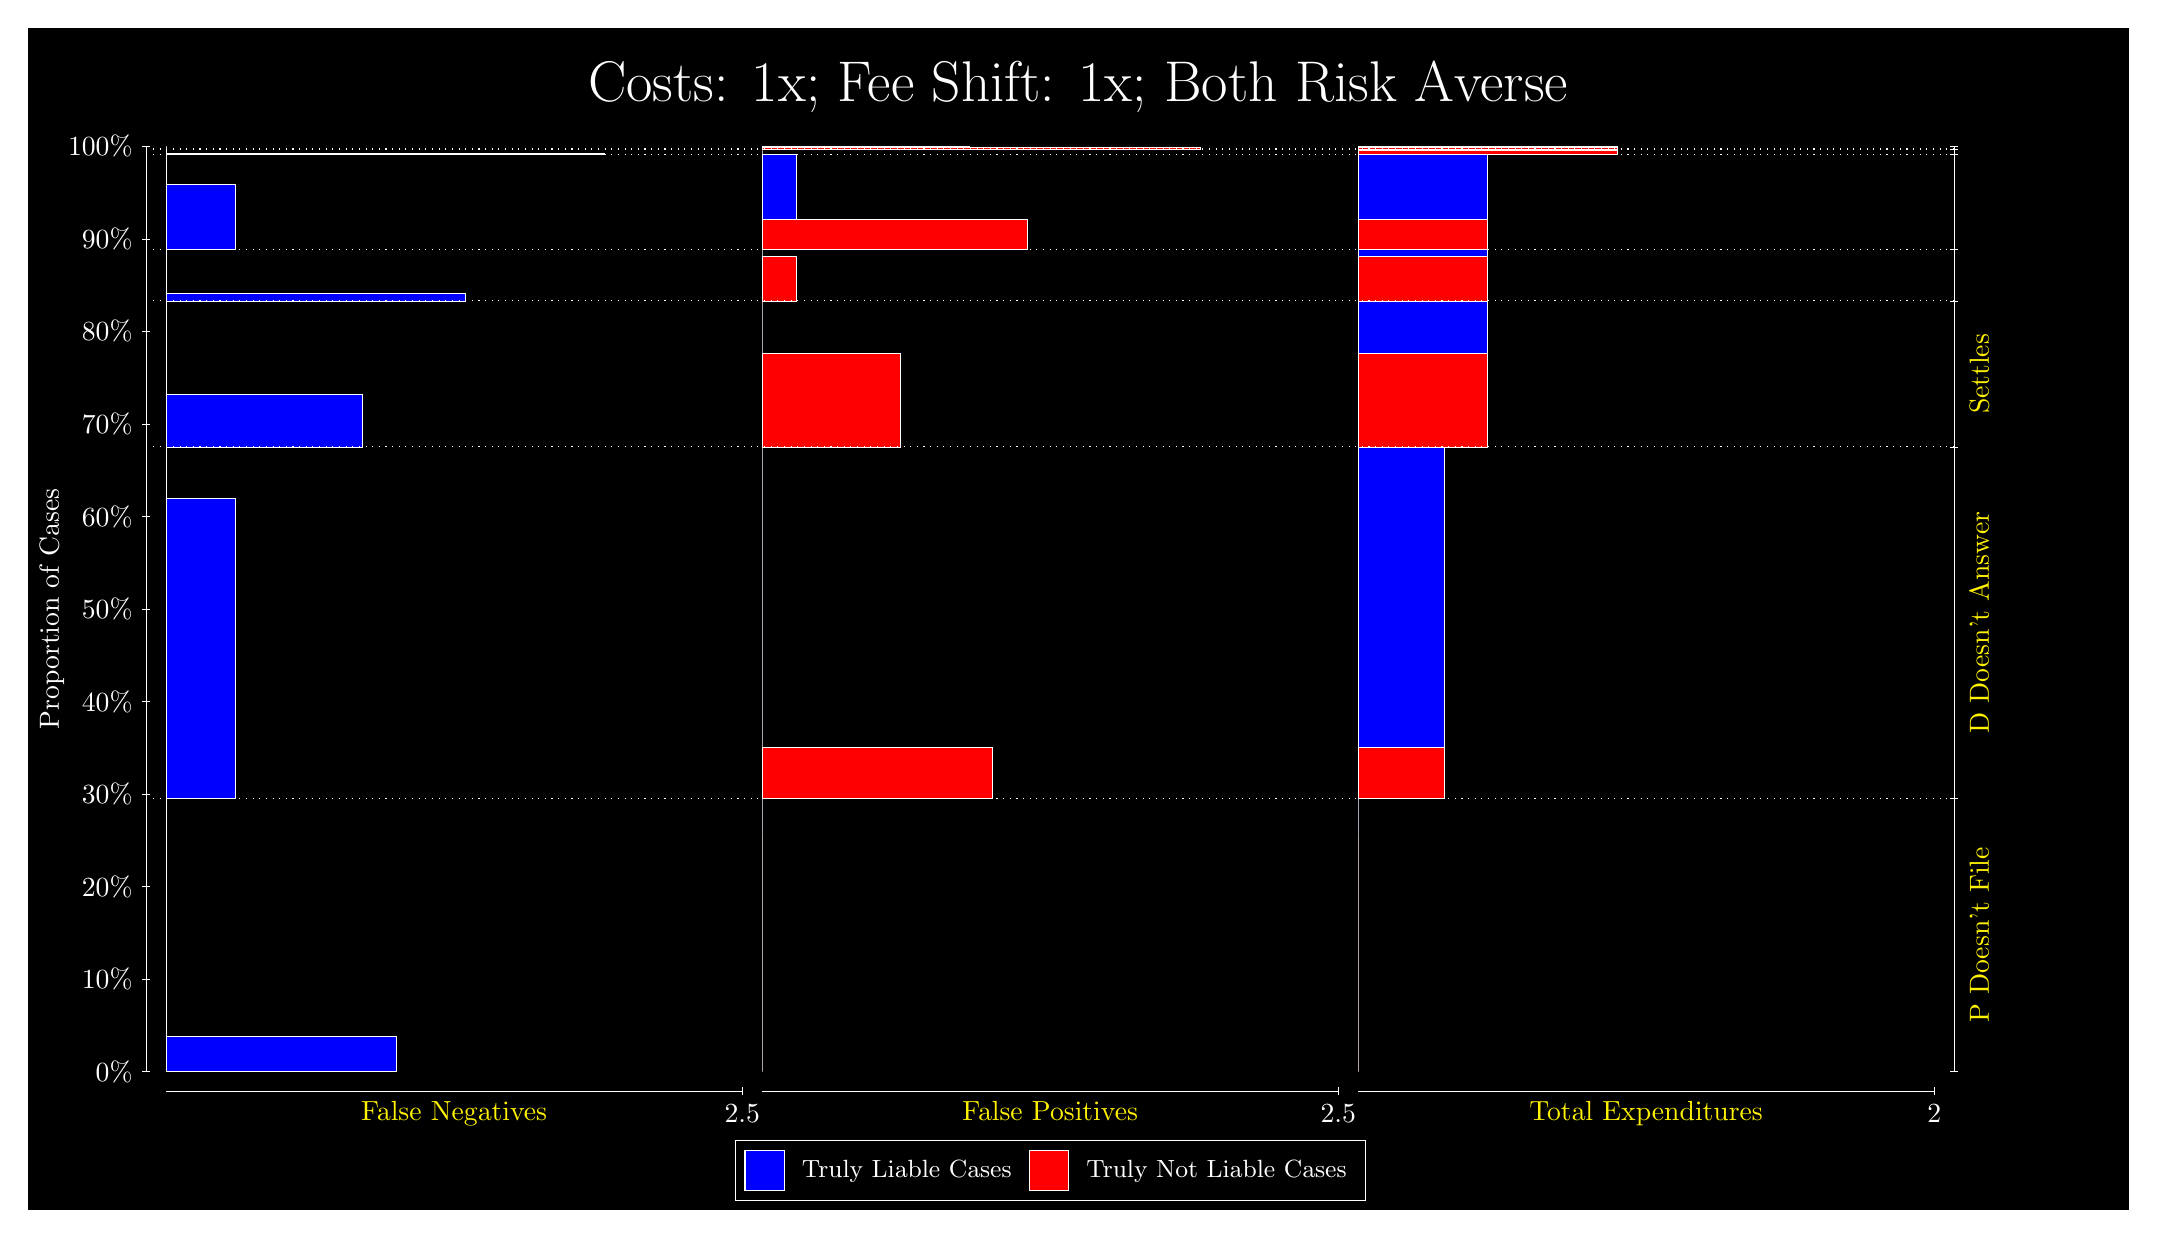
\begin{tikzpicture}
\draw[fill=black] (0,0) rectangle (26.667,15);
\draw[text=white] (0,13.5) rectangle (26.667,15) node[midway] {\huge Costs: 1x; Fee Shift: 1x; Both Risk Averse};
\draw[white, very thin] (1.5,1.75) -- (1.5,13.5);
\node[rotate=90, text=white, anchor=center] at (0.3, 7.625) {Proportion of Cases};
\draw[white, very thin] (1.45,1.75) -- (1.55,1.75);
\node[text=white, anchor=east] at (1.45, 1.75) {0\%};
\draw[white, very thin] (1.45,2.925) -- (1.55,2.925);
\node[text=white, anchor=east] at (1.45, 2.925) {10\%};
\draw[white, very thin] (1.45,4.1) -- (1.55,4.1);
\node[text=white, anchor=east] at (1.45, 4.1) {20\%};
\draw[white, very thin] (1.45,5.275) -- (1.55,5.275);
\node[text=white, anchor=east] at (1.45, 5.275) {30\%};
\draw[white, very thin] (1.45,6.45) -- (1.55,6.45);
\node[text=white, anchor=east] at (1.45, 6.45) {40\%};
\draw[white, very thin] (1.45,7.625) -- (1.55,7.625);
\node[text=white, anchor=east] at (1.45, 7.625) {50\%};
\draw[white, very thin] (1.45,8.8) -- (1.55,8.8);
\node[text=white, anchor=east] at (1.45, 8.8) {60\%};
\draw[white, very thin] (1.45,9.975) -- (1.55,9.975);
\node[text=white, anchor=east] at (1.45, 9.975) {70\%};
\draw[white, very thin] (1.45,11.15) -- (1.55,11.15);
\node[text=white, anchor=east] at (1.45, 11.15) {80\%};
\draw[white, very thin] (1.45,12.325) -- (1.55,12.325);
\node[text=white, anchor=east] at (1.45, 12.325) {90\%};
\draw[white, very thin] (1.45,13.5) -- (1.55,13.5);
\node[text=white, anchor=east] at (1.45, 13.5) {100\%};

\draw[white, very thin] (24.457,1.75) -- (24.457,13.5);
\draw[white, very thin] (24.407,1.75) -- (24.507,1.75);
\node[anchor=west] at (24.407, 1.75) {};
\draw[white, very thin] (24.407,5.2168) -- (24.507,5.2168);
\node[anchor=west] at (24.407, 5.2168) {};
\draw[white, very thin] (24.407,9.6834) -- (24.507,9.6834);
\node[anchor=west] at (24.407, 9.6834) {};
\draw[white, very thin] (24.407,11.537) -- (24.507,11.537);
\node[anchor=west] at (24.407, 11.537) {};
\draw[white, very thin] (24.407,12.194) -- (24.507,12.194);
\node[anchor=west] at (24.407, 12.194) {};
\draw[white, very thin] (24.407,13.399) -- (24.507,13.399);
\node[anchor=west] at (24.407, 13.399) {};
\draw[white, very thin] (24.407,13.466) -- (24.507,13.466);
\node[anchor=west] at (24.407, 13.466) {};
\draw[white, very thin] (24.407,13.5) -- (24.507,13.5);
\node[anchor=west] at (24.407, 13.5) {};

\draw[white, very thin, fill=blue] (1.75,1.75) rectangle (4.6775,2.1965);
\draw[white, very thin, fill=red] (1.75,2.1965) rectangle (1.75,5.2168);
\draw[white, very thin, fill=blue] (1.75,5.2168) rectangle (2.6283,9.0262);
\draw[white, very thin, fill=red] (1.75,9.0262) rectangle (1.75,9.6834);
\draw[white, very thin, fill=blue] (1.75,9.6834) rectangle (4.2384,10.347);
\draw[white, very thin, fill=red] (1.75,10.347) rectangle (1.75,11.537);
\draw[white, very thin, fill=blue] (1.75,11.537) rectangle (5.5558,11.63);
\draw[white, very thin, fill=red] (1.75,11.63) rectangle (1.75,12.194);
\draw[white, very thin, fill=blue] (1.75,12.194) rectangle (2.6283,13.023);
\draw[white, very thin, fill=red] (1.75,13.023) rectangle (1.75,13.399);
\draw[white, very thin, fill=blue] (1.75,13.399) rectangle (7.3123,13.416);
\draw[white, very thin, fill=red] (1.75,13.416) rectangle (1.75,13.466);
\draw[white, very thin, fill=red] (1.75,13.466) rectangle (1.75,13.482);
\draw[white, very thin, fill=blue] (1.75,13.482) rectangle (1.75,13.5);
\draw[white, very thin, fill=red] (9.3189,1.75) rectangle (9.3189,4.7704);
\draw[white, very thin, fill=blue] (9.3189,4.7704) rectangle (9.3189,5.2168);
\draw[white, very thin, fill=red] (9.3189,5.2168) rectangle (12.246,5.8739);
\draw[white, very thin, fill=blue] (9.3189,5.8739) rectangle (9.3189,9.6834);
\draw[white, very thin, fill=red] (9.3189,9.6834) rectangle (11.075,10.874);
\draw[white, very thin, fill=blue] (9.3189,10.874) rectangle (9.3189,11.537);
\draw[white, very thin, fill=red] (9.3189,11.537) rectangle (9.758,12.102);
\draw[white, very thin, fill=blue] (9.3189,12.102) rectangle (9.3189,12.194);
\draw[white, very thin, fill=red] (9.3189,12.194) rectangle (12.686,12.57);
\draw[white, very thin, fill=blue] (9.3189,12.57) rectangle (9.758,13.399);
\draw[white, very thin, fill=red] (9.3189,13.399) rectangle (9.3189,13.449);
\draw[white, very thin, fill=blue] (9.3189,13.449) rectangle (9.3189,13.466);
\draw[white, very thin, fill=red] (9.3189,13.466) rectangle (14.881,13.482);
\draw[white, very thin, fill=blue] (9.3189,13.482) rectangle (11.954,13.5);
\draw[white, very thin, fill=red] (16.888,1.75) rectangle (16.888,4.7704);
\draw[white, very thin, fill=blue] (16.888,4.7704) rectangle (16.888,5.2168);
\draw[white, very thin, fill=red] (16.888,5.2168) rectangle (17.986,5.8739);
\draw[white, very thin, fill=blue] (16.888,5.8739) rectangle (17.986,9.6834);
\draw[white, very thin, fill=red] (16.888,9.6834) rectangle (18.534,10.874);
\draw[white, very thin, fill=blue] (16.888,10.874) rectangle (18.534,11.537);
\draw[white, very thin, fill=red] (16.888,11.537) rectangle (18.534,12.102);
\draw[white, very thin, fill=blue] (16.888,12.102) rectangle (18.534,12.194);
\draw[white, very thin, fill=red] (16.888,12.194) rectangle (18.534,12.57);
\draw[white, very thin, fill=blue] (16.888,12.57) rectangle (18.534,13.399);
\draw[white, very thin, fill=red] (16.888,13.399) rectangle (20.181,13.449);
\draw[white, very thin, fill=blue] (16.888,13.449) rectangle (20.181,13.466);
\draw[white, very thin, fill=red] (16.888,13.466) rectangle (20.181,13.482);
\draw[white, very thin, fill=blue] (16.888,13.482) rectangle (20.181,13.5);
\draw[white, dotted] (1.5,5.2168) -- (24.457,5.2168);
\draw[white, dotted] (1.5,9.6834) -- (24.457,9.6834);
\draw[white, dotted] (1.5,11.537) -- (24.457,11.537);
\draw[white, dotted] (1.5,12.194) -- (24.457,12.194);
\draw[white, dotted] (1.5,13.399) -- (24.457,13.399);
\draw[white, dotted] (1.5,13.466) -- (24.457,13.466);
\draw[white, very thin] (1.75,1.5) -- (9.0689,1.5);
\node[text=yellow, anchor=north] at (5.4094, 1.5) {False Negatives};
\draw[white, very thin] (9.0689,1.45) -- (9.0689,1.55);
\node[text=white, anchor=north] at (9.0689, 1.45) {2.5};

\draw[white, very thin] (9.3189,1.5) -- (16.638,1.5);
\node[text=yellow, anchor=north] at (12.978, 1.5) {False Positives};
\draw[white, very thin] (16.638,1.45) -- (16.638,1.55);
\node[text=white, anchor=north] at (16.638, 1.45) {2.5};

\draw[white, very thin] (16.888,1.5) -- (24.207,1.5);
\node[text=yellow, anchor=north] at (20.547, 1.5) {Total Expenditures};
\draw[white, very thin] (24.207,1.45) -- (24.207,1.55);
\node[text=white, anchor=north] at (24.207, 1.45) {2};

\node[text=yellow, centered, rotate=90] at (24.777, 3.4834) {P Doesn't File};
\node[text=yellow, centered, rotate=90] at (24.777, 7.4501) {D Doesn't Answer};
\node[text=yellow, centered, rotate=90] at (24.777, 10.61) {Settles};





\draw (12.978300999999998,1.5) node[draw=none] (baseCoordinate) {};
\begin{scope}[align=center]
        \matrix[scale=0.5, draw=white, below=0.5cm of baseCoordinate, nodes={draw}, column sep=0.1cm]{
            \node[rectangle, draw, minimum width=0.5cm, minimum height=0.5cm, fill=blue] {}; &
            \node[draw=none, font=\small, text=white] (B) {Truly Liable Cases}; &
            \node[rectangle, draw, minimum width=0.5cm, minimum height=0.5cm, fill=red] {}; &
            \node[draw=none, font=\small, text=white] (B) {Truly Not Liable Cases}; \\
            };
\end{scope}

\end{tikzpicture}
\end{document}